
\documentclass[aspectratio=169,10pt]{beamer}

% -----------------------------------------------------------------------------
% intern02.tex
% Final internship presentation deck.
% This Beamer file is self-contained: it does not require external figures.
% -----------------------------------------------------------------------------

\usetheme{Frankfurt}
\setbeamertemplate{navigation symbols}{}
\setbeamertemplate{footline}[frame number]
\setbeamertemplate{headline}{}

\usepackage[T1]{fontenc}
\usepackage[utf8]{inputenc}
\usepackage{lmodern}
\usepackage{amsmath,amssymb}
\usepackage{booktabs}
\usepackage{array}
\usepackage{tabularx}
\usepackage{tikz}
\usetikzlibrary{arrows.meta,positioning,calc,fit,shapes.geometric,decorations.pathreplacing}
\usepackage{pgfplots}
\pgfplotsset{compat=1.18}

% Colors, close to intern01.
\definecolor{kepblue}{RGB}{42,88,140}
\definecolor{kepteal}{RGB}{33,132,120}
\definecolor{keporange}{RGB}{210,122,39}
\definecolor{kepred}{RGB}{178,61,68}
\definecolor{kepgray}{RGB}{92,99,112}
\definecolor{kepgreen}{RGB}{65,140,80}
\definecolor{keppurple}{RGB}{112,85,160}

\setbeamercolor{structure}{fg=kepblue}
\setbeamercolor{block title}{bg=kepblue!12,fg=kepblue!95!black}
\setbeamercolor{block body}{bg=kepblue!4,fg=black}
\setbeamercolor{alerted text}{fg=kepred}
\setbeamercolor{alertblock title}{bg=kepred!12,fg=kepred!90!black}
\setbeamercolor{alertblock body}{bg=kepred!4,fg=black}
\setbeamercolor{exampleblock title}{bg=kepteal!12,fg=kepteal!80!black}
\setbeamercolor{exampleblock body}{bg=kepteal!4,fg=black}

% Macros.
\newcommand{\V}{\mathcal{V}}
\newcommand{\A}{\mathcal{A}}
\newcommand{\RDP}{\mathcal{R}}
\newcommand{\NDD}{\mathcal{N}}
\newcommand{\Y}{\mathcal{Y}}
\newcommand{\wtrue}{w^{\mathrm{true}}}
\newcommand{\what}{\widehat{w}}
\newcommand{\ystar}{y^{\star}}
\newcommand{\ytwo}{y_{\mathrm{2stage}}}
\newcommand{\gap}{\operatorname{gap}}
\DeclareMathOperator*{\argmax}{arg\,max}

% TikZ styles. Prefix names to avoid collision with Beamer block environments.
\tikzset{
  kcard/.style={draw=kepblue!70, fill=kepblue!6, rounded corners=2pt, align=center,
    minimum height=8mm, text width=28mm, font=\small},
  kcardwide/.style={draw=kepblue!70, fill=kepblue!6, rounded corners=2pt, align=center,
    minimum height=9mm, text width=42mm, font=\small},
  ksmall/.style={draw=kepgray!70, fill=kepgray!7, rounded corners=2pt, align=center,
    minimum height=7mm, text width=24mm, font=\scriptsize},
  korange/.style={draw=keporange!80, fill=keporange!8, rounded corners=2pt, align=center,
    minimum height=8mm, text width=32mm, font=\small},
  kgreen/.style={draw=kepgreen!80!black, fill=kepgreen!8, rounded corners=2pt, align=center,
    minimum height=8mm, text width=32mm, font=\small},
  kred/.style={draw=kepred!80, fill=kepred!8, rounded corners=2pt, align=center,
    minimum height=8mm, text width=32mm, font=\small},
  pair/.style={circle, draw=kepblue!80, fill=kepblue!8, minimum size=8.5mm,
    inner sep=1pt, font=\scriptsize},
  ndd/.style={circle, draw=kepteal!90!black, fill=kepteal!10, minimum size=8.5mm,
    inner sep=1pt, font=\scriptsize},
  arr/.style={-Latex, thick, kepblue!85},
  grayarr/.style={-Latex, thick, kepgray!75},
  highlightarr/.style={-Latex, very thick, keporange},
  goodarr/.style={-Latex, very thick, kepgreen!80!black},
  badarr/.style={-Latex, very thick, kepred!85!black}
}

\title{Decision-Focused Learning for Kidney Exchange Programs}
\subtitle{When Does It Help?}
\author{Weikang Fu}
\institute{MILA \\ Universit\'{e} de Montr\'{e}al}
\date{Final Internship Presentation}

\begin{document}

% -----------------------------------------------------------------------------
% Main presentation: designed for ~12 minutes.
% -----------------------------------------------------------------------------

\begin{frame}
  \titlepage
  \vspace{-1.2em}
  \begin{center}
    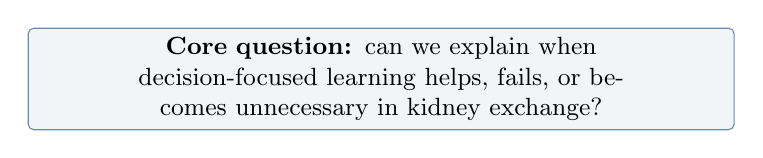
\begin{tikzpicture}
      \node[kcardwide,text width=0.72\textwidth] {
        \textbf{Core question:} can we explain when decision-focused learning helps, fails, or becomes unnecessary in kidney exchange?
      };
    \end{tikzpicture}
  \end{center}
\end{frame}

\section{From Question to Mechanism}

\begin{frame}{From ``Can DFL Help?'' to ``When Does DFL Help?''}
  \small
  \begin{columns}[T,onlytextwidth]
    \begin{column}{0.47\textwidth}
      \begin{block}{First presentation}
        \textbf{Question}\\
        Can decision-focused learning improve controlled KEP decisions?

        \vspace{0.7em}
        \textbf{Finding}\\
        Promising signal, but not robust enough yet.
      \end{block}
    \end{column}

    \begin{column}{0.47\textwidth}
      \begin{exampleblock}{Final presentation}
        \textbf{Question}\\
        When does DFL help, fail, or become unnecessary?

        \vspace{0.7em}
        \textbf{Answer}\\
        It is a candidate-reranking effect inside the feasible exchange landscape.
      \end{exampleblock}
    \end{column}
  \end{columns}

  \vspace{0.8em}
  \begin{alertblock}{Main shift}
    \centering
    From \textbf{method comparison} to \textbf{mechanism understanding}.
  \end{alertblock}
\end{frame}

\begin{frame}{Recap: Kidney Exchange as a Weighted Decision Problem}
  \footnotesize
  \begin{columns}[T,onlytextwidth]
    \begin{column}{0.42\textwidth}
      \begin{block}{Input}
        A directed compatibility graph with recipient--donor pairs and non-directed donors.
      \end{block}
      \begin{block}{Decision}
        Select vertex-disjoint cycles and chains under length limits.
      \end{block}
      \begin{block}{Objective}
        Maximize total predicted transplant benefit.
      \end{block}
    \end{column}

    \begin{column}{0.55\textwidth}
      \centering
      \resizebox{0.95\linewidth}{!}{%
      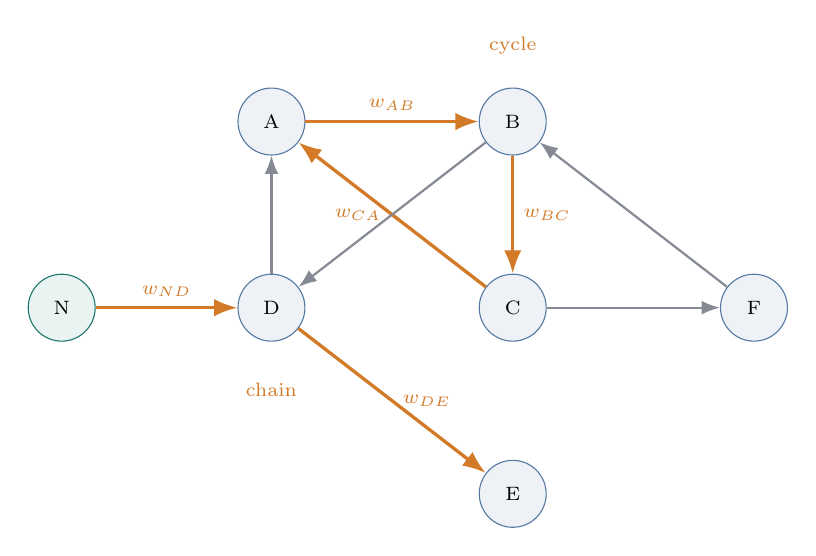
\begin{tikzpicture}[node distance=15mm]
        \node[pair] (a) {A};
        \node[pair,right=22mm of a] (b) {B};
        \node[pair,below=15mm of b] (c) {C};
        \node[pair,below=15mm of a] (d) {D};
        \node[ndd,left=18mm of d] (n) {N};
        \node[pair,below=15mm of c] (e) {E};
        \node[pair,right=22mm of c] (f) {F};

        \draw[highlightarr] (a) -- node[above,font=\scriptsize] {$w_{AB}$} (b);
        \draw[highlightarr] (b) -- node[right,font=\scriptsize] {$w_{BC}$} (c);
        \draw[highlightarr] (c) -- node[left,font=\scriptsize] {$w_{CA}$} (a);
        \draw[grayarr] (d) -- (a);
        \draw[grayarr] (b) -- (d);
        \draw[highlightarr] (n) -- node[above,font=\scriptsize] {$w_{ND}$} (d);
        \draw[highlightarr] (d) -- node[right,font=\scriptsize] {$w_{DE}$} (e);
        \draw[grayarr] (c) -- (f);
        \draw[grayarr] (f) -- (b);

        \node[font=\scriptsize,keporange,above=3mm of b] {cycle};
        \node[font=\scriptsize,keporange,below=4mm of d] {chain};
      \end{tikzpicture}}

      \vspace{0.4em}
      \scriptsize
      The learning model predicts edge weights; the optimizer chooses the exchange plan.
    \end{column}
  \end{columns}
\end{frame}

\begin{frame}{Prediction Accuracy Is Not the Final Goal}
  \small
  \centering
  \resizebox{0.93\textwidth}{!}{%
  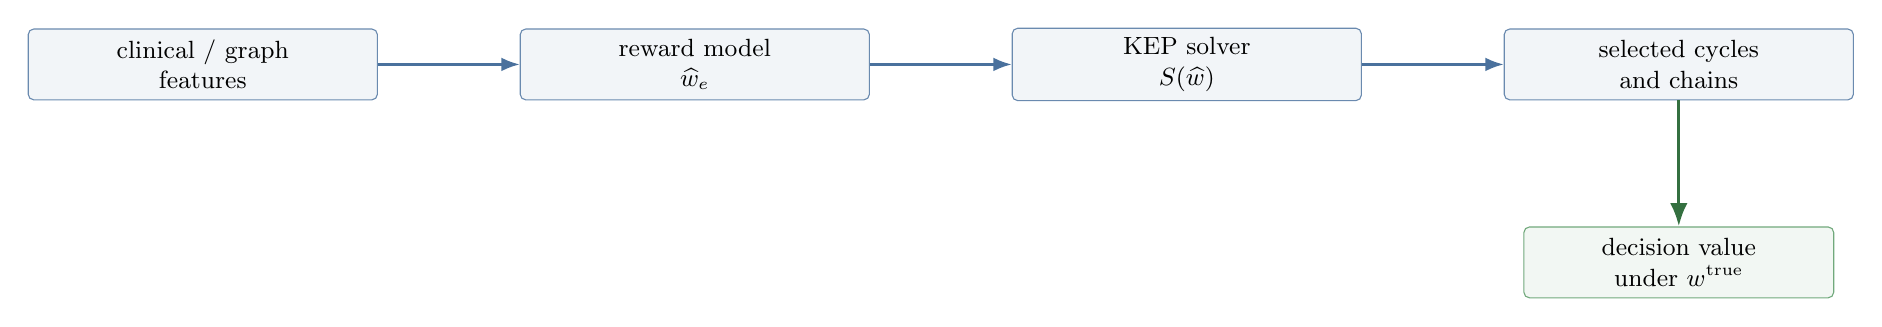
\begin{tikzpicture}[node distance=15mm]
    \node[kcardwide] (features) {clinical / graph\\features};
    \node[kcardwide,right=18mm of features] (model) {reward model\\$\widehat{w}_e$};
    \node[kcardwide,right=18mm of model] (solver) {KEP solver\\$S(\widehat{w})$};
    \node[kcardwide,right=18mm of solver] (plan) {selected cycles\\and chains};
    \node[kcardwide,below=16mm of plan,text width=37mm,draw=kepgreen!75,fill=kepgreen!7] (value) {decision value\\under $w^{\mathrm{true}}$};

    \draw[arr] (features) -- (model);
    \draw[arr] (model) -- (solver);
    \draw[arr] (solver) -- (plan);
    \draw[goodarr] (plan) -- (value);
  \end{tikzpicture}}

  \vspace{0.7em}
  \begin{columns}[T,onlytextwidth]
    \begin{column}{0.46\textwidth}
      \begin{block}{Two-stage learning}
        \centering
        Fit edge rewards first, then optimize.
      \end{block}
    \end{column}
    \begin{column}{0.46\textwidth}
      \begin{exampleblock}{Decision-focused learning}
        \centering
        Train for downstream decision quality.
      \end{exampleblock}
    \end{column}
  \end{columns}

  \vspace{0.4em}
  \begin{alertblock}{New observation}
    \centering
    In KEP, a \textbf{different} selected plan is not always a \textbf{bad} selected plan.
  \end{alertblock}
\end{frame}

\section{Core Hypothesis}

\begin{frame}{Key Hypothesis: Close Substitute Solutions}
  \small
  \centering
  \begin{block}{Hypothesis}
    \centering
    Kidney exchange often contains many \textbf{close substitute exchange plans}.
  \end{block}

  \vspace{0.4em}
  \begin{columns}[T,onlytextwidth]
    \begin{column}{0.50\textwidth}
      \textbf{Why KEP can behave this way}
      \begin{itemize}\setlength{\itemsep}{0.45em}
        \item A feasible plan is a packing of cycles and chains.
        \item One exchange can often be replaced by another.
        \item The plan identity changes, but its objective value may stay close.
      \end{itemize}

      \vspace{0.35em}
      \centering
      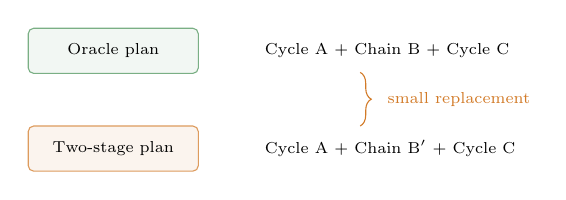
\begin{tikzpicture}[scale=0.82, every node/.style={transform shape}]
        \node[ksmall,draw=kepgreen!70,fill=kepgreen!7] (o1) at (0,0) {Oracle plan};
        \node[ksmall,below=8mm of o1,draw=keporange!75,fill=keporange!8] (t1) {Two-stage plan};
        \node[font=\scriptsize,right=9mm of o1] (otext) {Cycle A + Chain B + Cycle C};
        \node[font=\scriptsize,right=9mm of t1] (ttext) {Cycle A + Chain B$'$ + Cycle C};
        \draw[decorate,decoration={brace,amplitude=4pt},keporange] ($(otext.south west)+(16mm,-1mm)$) -- ($(ttext.north west)+(16mm,1mm)$)
          node[midway,right=3mm,font=\scriptsize,keporange] {small replacement};
      \end{tikzpicture}
    \end{column}

    \begin{column}{0.45\textwidth}
      \textbf{Simple implication}
      \[
        \gap(\ytwo) \le \epsilon
      \]
      \[
        \Longrightarrow
        \text{max possible improvement} \le \epsilon .
      \]

      \vspace{0.5em}
      \begin{alertblock}{Interpretation}
        \centering
        DFL can only remove regret that is actually present.
      \end{alertblock}
    \end{column}
  \end{columns}
\end{frame}

\begin{frame}{Looking Beyond the Best Predicted Solution}
  \small
  \begin{columns}[T,onlytextwidth]
    \begin{column}{0.48\textwidth}
      \begin{block}{Diagnostic idea}
        For each trained model and graph:
        \begin{enumerate}\setlength{\itemsep}{0.25em}
          \item Find the best predicted KEP solution.
          \item Exclude it with a no-good cut.
          \item Re-solve for the next distinct solution.
          \item Evaluate both under the true synthetic reward.
        \end{enumerate}
      \end{block}

      \begin{alertblock}{Question}
        \centering
        If rank 1 is removed, does the next solution collapse, or remain near-oracle?
      \end{alertblock}
    \end{column}

    \begin{column}{0.48\textwidth}
      \centering
      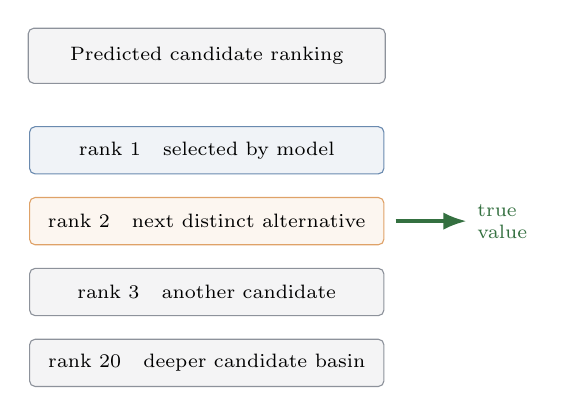
\begin{tikzpicture}[x=1mm,y=1mm]
        \node[ksmall,text width=43mm] at (25,48) {Predicted candidate ranking};
        \node[draw=kepblue!70,fill=kepblue!7,rounded corners=2pt,minimum width=45mm,minimum height=6mm,align=left,font=\scriptsize] at (25,36) {rank 1\quad selected by model};
        \node[draw=keporange!70,fill=keporange!7,rounded corners=2pt,minimum width=45mm,minimum height=6mm,align=left,font=\scriptsize] at (25,27) {rank 2\quad next distinct alternative};
        \node[draw=kepgray!70,fill=kepgray!7,rounded corners=2pt,minimum width=45mm,minimum height=6mm,align=left,font=\scriptsize] at (25,18) {rank 3\quad another candidate};
        \node[draw=kepgray!70,fill=kepgray!7,rounded corners=2pt,minimum width=45mm,minimum height=6mm,align=left,font=\scriptsize] at (25,9) {rank 20\quad deeper candidate basin};
        \draw[goodarr] (49,27) -- (58,27) node[right,font=\scriptsize,align=left] {true\\value};
      \end{tikzpicture}
    \end{column}
  \end{columns}
\end{frame}

\section{Findings}

\begin{frame}{Finding 1: Many Second-Best Solutions Are Still Good}
  \small
  \begin{columns}[T,onlytextwidth]
    \begin{column}{0.48\textwidth}
      \begin{block}{2stage rank 2}
        \centering
        {\Large\textbf{7.04\%}}\\[-0.1em]
        {\scriptsize mean normalized oracle gap}

        \vspace{0.55em}
        {\Large\textbf{45.19\%}}\\[-0.1em]
        {\scriptsize within 5\% of oracle}
      \end{block}
    \end{column}

    \begin{column}{0.48\textwidth}
      \begin{exampleblock}{SPO+ rank 2}
        \centering
        {\Large\textbf{6.32\%}}\\[-0.1em]
        {\scriptsize mean normalized oracle gap}

        \vspace{0.55em}
        {\Large\textbf{47.97\%}}\\[-0.1em]
        {\scriptsize within 5\% of oracle}
      \end{exampleblock}
    \end{column}
  \end{columns}

  \vspace{0.6em}
  \begin{center}
  \begin{tikzpicture}
    \begin{axis}[
      ybar,
      width=0.78\textwidth,
      height=0.25\textheight,
      ymin=0, ymax=65,
      ylabel={within 5\% rate},
      symbolic x coords={2stage r1,2stage r2,SPO+ r1,SPO+ r2},
      xtick=data,
      x tick label style={font=\scriptsize, align=center},
      yticklabel={\pgfmathprintnumber{\tick}\%},
      nodes near coords={\pgfmathprintnumber[fixed,precision=1]{\pgfplotspointmeta}\%},
      nodes near coords align={vertical},
      bar width=10pt,
      tick label style={font=\scriptsize},
      label style={font=\scriptsize},
      every node near coord/.append style={font=\tiny},
      enlarge x limits=0.17,
      axis y line*=left,
      axis x line*=bottom,
    ]
      \addplot[fill=kepblue!35,draw=kepblue!85] coordinates {
        (2stage r1,53.14) (2stage r2,45.19) (SPO+ r1,59.28) (SPO+ r2,47.97)
      };
    \end{axis}
  \end{tikzpicture}
  \end{center}

  \begin{alertblock}{Interpretation}
    \centering
    Excluding the best predicted solution often still leaves a near-oracle alternative.
  \end{alertblock}
\end{frame}

\begin{frame}{Why Average DFL Gains Can Be Moderate}
  \small
  \begin{columns}[T,onlytextwidth]
    \begin{column}{0.46\textwidth}
      \begin{block}{When two-stage is bad}
        \centering
        DFL has room to help.
      \end{block}
      \centering
      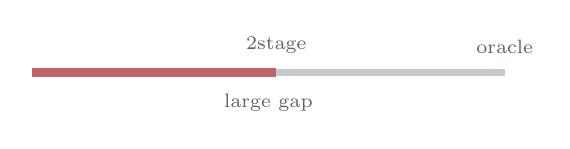
\begin{tikzpicture}[x=1mm,y=1mm]
        \draw[line width=2.3pt,kepgray!35] (0,0) -- (60,0);
        \draw[line width=3.3pt,kepred!80] (0,0) -- (31,0);
        \node[font=\scriptsize,kepgray,below] at (30,-1.5) {large gap};
        \node[font=\scriptsize,kepgray,above] at (60,1.2) {oracle};
        \node[font=\scriptsize,kepgray,above] at (31,1.2) {2stage};
      \end{tikzpicture}
    \end{column}

    \begin{column}{0.46\textwidth}
      \begin{exampleblock}{When two-stage is close}
        \centering
        Little regret remains to remove.
      \end{exampleblock}
      \centering
      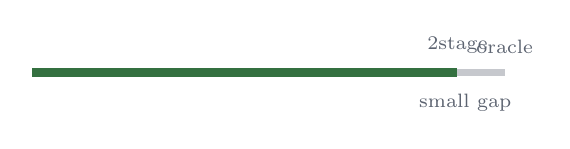
\begin{tikzpicture}[x=1mm,y=1mm]
        \draw[line width=2.3pt,kepgray!35] (0,0) -- (60,0);
        \draw[line width=3.3pt,kepgreen!80!black] (0,0) -- (54,0);
        \node[font=\scriptsize,kepgray,below] at (55,-1.5) {small gap};
        \node[font=\scriptsize,kepgray,above] at (60,1.2) {oracle};
        \node[font=\scriptsize,kepgray,above] at (54,1.2) {2stage};
      \end{tikzpicture}
    \end{column}
  \end{columns}

  \vspace{1.1em}
  \begin{alertblock}{Ceiling effect}
    \centering
    If the two-stage plan is already a close substitute, even a perfect DFL method\\ can only improve a little.
  \end{alertblock}

  \vspace{0.3em}
  \centering
  \begin{minipage}{0.88\textwidth}\centering\scriptsize This explains why KEP can have many solution-identity errors but only moderate average regret improvements.\end{minipage}
\end{frame}

\begin{frame}{Finding 2: SPO+ Often Reranks Existing Candidates}
  \small
  \begin{columns}[T,onlytextwidth]
    \begin{column}{0.49\textwidth}
      \textbf{Two-stage predicted ranking}
      \vspace{0.4em}

      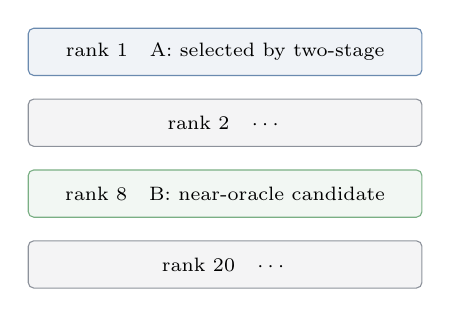
\begin{tikzpicture}[x=1mm,y=1mm]
        \node[draw=kepblue!70,fill=kepblue!7,rounded corners=2pt,minimum width=50mm,minimum height=6mm,align=left,font=\scriptsize] at (27,35) {rank 1\quad A: selected by two-stage};
        \node[draw=kepgray!70,fill=kepgray!7,rounded corners=2pt,minimum width=50mm,minimum height=6mm,align=left,font=\scriptsize] at (27,26) {rank 2\quad $\cdots$};
        \node[draw=kepgreen!70,fill=kepgreen!7,rounded corners=2pt,minimum width=50mm,minimum height=6mm,align=left,font=\scriptsize] at (27,17) {rank 8\quad B: near-oracle candidate};
        \node[draw=kepgray!70,fill=kepgray!7,rounded corners=2pt,minimum width=50mm,minimum height=6mm,align=left,font=\scriptsize] at (27,8) {rank 20\quad $\cdots$};
      \end{tikzpicture}
    \end{column}

    \begin{column}{0.48\textwidth}
      \textbf{SPO+ selected ranking}
      \vspace{0.4em}

      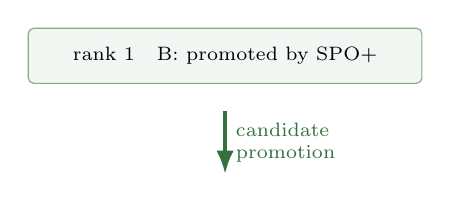
\begin{tikzpicture}[x=1mm,y=1mm]
        \node[draw=kepgreen!70,fill=kepgreen!7,rounded corners=2pt,minimum width=50mm,minimum height=7mm,align=left,font=\scriptsize] at (27,35) {rank 1\quad B: promoted by SPO+};
        \draw[goodarr] (27,28) -- (27,20) node[midway,right,font=\scriptsize,align=left] {candidate\\promotion};
      \end{tikzpicture}

      \vspace{0.2em}
      \begin{block}{Successful reranking}
        \centering
        The promoted candidate is near-oracle.
      \end{block}

      \begin{alertblock}{Harmful reranking}
        \centering
        The promoted candidate is not near-oracle.
      \end{alertblock}
    \end{column}
  \end{columns}

  \vspace{0.3em}
  \centering
  {\scriptsize Same mechanism; different candidate quality.}
\end{frame}

\begin{frame}{Case Examples: Correction, Promotion, and Harmful Reranking}
  \footnotesize
  \begin{columns}[T,onlytextwidth]
    \begin{column}{0.31\textwidth}
      \begin{exampleblock}{G-1285}
        \textbf{Clean rank-2 promotion}
        \vspace{0.35em}
        \begin{itemize}\setlength{\itemsep}{0.35em}
          \item SPO+ rank 1 equals two-stage rank 2.
          \item Promoted solution equals true oracle top 1.
          \item Cleanest success case.
        \end{itemize}
      \end{exampleblock}
    \end{column}

    \begin{column}{0.31\textwidth}
      \begin{block}{G-392}
        \textbf{Deep-candidate correction}
        \vspace{0.35em}
        \begin{itemize}\setlength{\itemsep}{0.35em}
          \item Two-stage contains a near-oracle candidate.
          \item But it appears around rank 8.
          \item SPO+ promotes it to rank 1.
        \end{itemize}
      \end{block}
    \end{column}

    \begin{column}{0.31\textwidth}
      \begin{alertblock}{G-14}
        \textbf{Harmful reranking}
        \vspace{0.35em}
        \begin{itemize}\setlength{\itemsep}{0.35em}
          \item SPO+ also promotes a lower-ranked candidate.
          \item But the promoted candidate is worse under true reward.
          \item Reranking is risky.
        \end{itemize}
      \end{alertblock}
    \end{column}
  \end{columns}

  \vspace{0.7em}
  \centering
  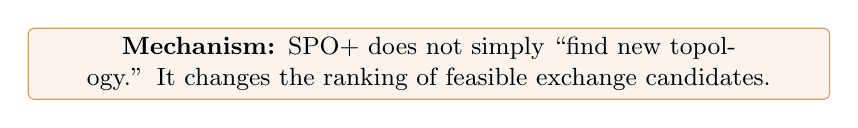
\begin{tikzpicture}
    \node[kcardwide,text width=0.82\textwidth,draw=keporange!75,fill=keporange!8] {
      \textbf{Mechanism:} SPO+ does not simply ``find new topology.'' It changes the ranking of feasible exchange candidates.
    };
  \end{tikzpicture}
\end{frame}

\begin{frame}{Ambiguity Means Opportunity and Risk}
  \small
  \begin{columns}[T,onlytextwidth]
    \begin{column}{0.44\textwidth}
      \begin{block}{Prediction-boundary ambiguity}
        \begin{itemize}\setlength{\itemsep}{0.35em}
          \item small top-1 / top-$k$ margin
          \item many near-tied candidates
          \item diverse top-$k$ solutions
          \item unstable rank-1 identity across seeds
        \end{itemize}
      \end{block}
    \end{column}

    \begin{column}{0.52\textwidth}
      \begin{exampleblock}{Interpretation}
        High ambiguity means DFL reranking can matter.
      \end{exampleblock}
      \begin{alertblock}{But}
        It does not say whether reranking will help or hurt.
      \end{alertblock}

      \vspace{0.2em}
      \centering
      \begin{tikzpicture}
        \begin{axis}[
          ybar,
          width=0.92\linewidth,
          height=0.28\textheight,
          ymin=0.45,ymax=0.82,
          ylabel={AUROC},
          symbolic x coords={top5 helpful,top5 harmful,top20 helpful,top20 harmful},
          xtick=data,
          x tick label style={font=\tiny, align=center, rotate=0},
          nodes near coords={\pgfmathprintnumber[fixed,precision=3]{\pgfplotspointmeta}},
          every node near coord/.append style={font=\tiny},
          bar width=9pt,
          tick label style={font=\scriptsize},
          label style={font=\scriptsize},
          enlarge x limits=0.13,
          axis y line*=left,
          axis x line*=bottom,
        ]
          \addplot[fill=kepblue!35,draw=kepblue!85] coordinates {
            (top5 helpful,0.715) (top5 harmful,0.577) (top20 helpful,0.739) (top20 harmful,0.732)
          };
        \end{axis}
      \end{tikzpicture}
    \end{column}
  \end{columns}
\end{frame}

\section{Takeaways}

\begin{frame}{Takeaways: DFL Is Useful, but Conditional}
  \scriptsize
  \begin{columns}[T,onlytextwidth]
    \begin{column}{0.31\textwidth}
      \begin{exampleblock}{What worked}
        \begin{itemize}\setlength{\itemsep}{0.35em}
          \item DFL can improve controlled KEP decisions.
          \item SPO+ gives stronger held-out gains than the earlier FY probe.
          \item It can correct decision-critical ranking errors.
        \end{itemize}
      \end{exampleblock}
    \end{column}

    \begin{column}{0.31\textwidth}
      \begin{block}{What changed}
        \begin{itemize}\setlength{\itemsep}{0.35em}
          \item The main question is no longer only: ``Does DFL beat MSE?''
          \item It is: ``When is there regret left for DFL to remove?''
          \item Mechanism matters as much as average performance.
        \end{itemize}
      \end{block}
    \end{column}

    \begin{column}{0.31\textwidth}
      \begin{alertblock}{What remains}
        \begin{itemize}\setlength{\itemsep}{0.35em}
          \item clinical reward models
          \item prospective diagnostics
          \item cross-regime robustness
          \item safer use when reranking is risky
        \end{itemize}
      \end{alertblock}
    \end{column}
  \end{columns}

  \vspace{0.8em}
  \begin{center}
    \colorbox{kepblue!8}{%
      \parbox{0.88\textwidth}{\centering\small
        \textbf{Conclusion:} In KEP, DFL is best understood as mechanism-aware candidate reranking, not as a universal replacement for predict-then-optimize.
      }%
    }
  \end{center}
\end{frame}

% -----------------------------------------------------------------------------
% Backup / appendix slides for Q&A.
% -----------------------------------------------------------------------------

\appendix
\section{Backup Slides}

\begin{frame}{Backup: KEP Mathematical Setup}
  \small
  \begin{columns}[T,onlytextwidth]
    \begin{column}{0.48\textwidth}
      \begin{block}{Compatibility graph}
        \[
          G=(\V,\A), \qquad \V = \RDP \cup \NDD
        \]
        \begin{itemize}\setlength{\itemsep}{0.25em}
          \item $\RDP$: incompatible recipient--donor pairs
          \item $\NDD$: non-directed donors
          \item $(u,v)\in\A$: donor at $u$ can donate to recipient at $v$
        \end{itemize}
      \end{block}
    \end{column}

    \begin{column}{0.48\textwidth}
      \begin{block}{Decision oracle}
        \[
          S(w) \in \argmax_{y\in\Y(G;K,L)} w^\top y
        \]
        \begin{itemize}\setlength{\itemsep}{0.25em}
          \item $K$: maximum cycle length
          \item $L$: maximum chain length
          \item $y$: selected edge-incidence vector
        \end{itemize}
      \end{block}
    \end{column}
  \end{columns}

  \vspace{0.6em}
  \begin{alertblock}{Learning challenge}
    \centering
    The oracle is combinatorial and piecewise constant in the predicted weights.
  \end{alertblock}
\end{frame}

\begin{frame}{Backup: Synthetic-Label Decision Gap}
  \small
  \begin{block}{Evaluation metric}
    \[
      \ystar = S(\wtrue), \qquad \widehat{y} = S(\what)
    \]
    \[
      \gap(\widehat{y})
      =
      (\wtrue)^\top \ystar - (\wtrue)^\top \widehat{y}
    \]
    \[
      \text{normalized gap}
      =
      \frac{(\wtrue)^\top \ystar - (\wtrue)^\top \widehat{y}}
           {|(\wtrue)^\top \ystar|}
    \]
  \end{block}

  \begin{alertblock}{Important boundary}
    \centering
    The ``true'' reward here is a synthetic benchmark label, not a clinical outcome.
  \end{alertblock}
\end{frame}

\begin{frame}{Backup: Robustness Lessons from the First Generalization Study}
  \scriptsize
  \begin{columns}[T,onlytextwidth]
    \begin{column}{0.47\textwidth}
      \begin{block}{Unseen 1000 graphs}
        \begin{itemize}\setlength{\itemsep}{0.3em}
          \item Strong FY gains on the original held-out split did not replicate cleanly.
          \item Two-stage baseline was very stable across train sizes.
          \item Many methods selected identical KEP decisions on most unseen graphs.
        \end{itemize}
      \end{block}
    \end{column}

    \begin{column}{0.47\textwidth}
      \begin{alertblock}{Realistic-synthetic label shift}
        \begin{itemize}\setlength{\itemsep}{0.3em}
          \item Two-stage was tied or slightly better across completed train sizes.
          \item Controlled noisy-linear training did not transfer cleanly to the more complex synthetic reward definition.
        \end{itemize}
      \end{alertblock}
    \end{column}
  \end{columns}

  \vspace{0.7em}
  \centering
  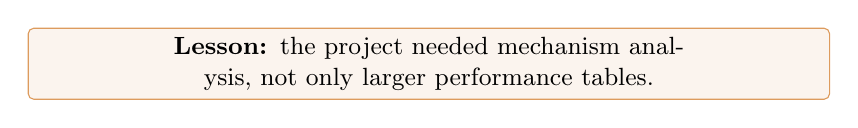
\begin{tikzpicture}
    \node[kcardwide,text width=0.82\textwidth,draw=keporange!75,fill=keporange!8] {
      \textbf{Lesson:} the project needed mechanism analysis, not only larger performance tables.
    };
  \end{tikzpicture}
\end{frame}

\begin{frame}{Backup: Strict SPO+ Surrogate Ablation}
  \scriptsize
  \begin{block}{Golden rule}
    \centering
    Only change the surrogate; keep the data, split, model class, initialization, training budget, checkpoint protocol, and evaluation metrics fixed.
  \end{block}

  \vspace{0.3em}
  \centering
  \begin{tabular}{@{}rrrrr@{}}
    \toprule
    train size & 2stage gap & SPO+ gap & improvement & 95\% CI \\
    \midrule
    50   & 0.8480 & 0.7401 & 0.1079 & [0.0347, 0.1960] \\
    200  & 0.8451 & 0.7706 & 0.0745 & [0.0170, 0.1527] \\
    600  & 0.8223 & 0.7706 & 0.0517 & [0.0044, 0.1112] \\
    1200 & 0.8441 & 0.7846 & 0.0594 & [0.0033, 0.1312] \\
    \bottomrule
  \end{tabular}

  \vspace{0.6em}
  \begin{alertblock}{Reading the table}
    \centering
    Held-out400 results for the validation-SPO+-loss checkpoint; lower gap is better.
  \end{alertblock}
\end{frame}

\begin{frame}{Backup: SPO+ Correctness Checks}
  \scriptsize
  \begin{columns}[T,onlytextwidth]
    \begin{column}{0.48\textwidth}
      \begin{exampleblock}{Shortest-path benchmark}
        \begin{itemize}\setlength{\itemsep}{0.35em}
          \item Oracle/objective alignment
          \item two-stage LR alignment
          \item SPO+ forward-loss alignment
          \item gradient and one-step SGD update alignment
        \end{itemize}
        \vspace{0.3em}
        \centering
        \textbf{Differences: around $10^{-6}$ or below}
      \end{exampleblock}
    \end{column}

    \begin{column}{0.48\textwidth}
      \begin{block}{KEP integration preflight}
        \begin{itemize}\setlength{\itemsep}{0.35em}
          \item reward-max / cost-min adapter
          \item same cached KEP solver wrapper
          \item loss and gradient agreement
          \item graph-specific edge-selection vectors
        \end{itemize}
        \vspace{0.3em}
        \centering
        \textbf{Phase-0 max absolute diffs: 0}
      \end{block}
    \end{column}
  \end{columns}
\end{frame}

\begin{frame}{Backup: Cycle-Length Sensitivity}
  \scriptsize
  \centering
  \begin{tabular}{@{}llrrr@{}}
    \toprule
    $K$ & method & rank-2 mean gap & rank-2 median gap & within 5\% \\
    \midrule
    3 & 2stage & 7.04\% & 5.75\% & 45.19\% \\
    4 & 2stage & 6.93\% & 5.53\% & 47.50\% \\
    5 & 2stage & 6.88\% & 5.20\% & 48.94\% \\
    3 & SPO+ & 6.32\% & 5.28\% & 47.97\% \\
    4 & SPO+ & 6.20\% & 5.03\% & 49.78\% \\
    5 & SPO+ & 5.61\% & 4.39\% & 54.83\% \\
    \bottomrule
  \end{tabular}

  \vspace{0.8em}
  \begin{block}{Interpretation}
    \centering
    The close-rank-2 behavior is not only an artifact of the max-cycle-3 feasible set.
  \end{block}
\end{frame}

\begin{frame}{Backup: Mechanism Atlas for Selected Cases}
  \scriptsize
  \centering
  \begin{tabularx}{0.98\textwidth}{@{}lXrrrr@{}}
    \toprule
    graph & updated mechanism & B found & SPO+=B & C rank & true $\Delta$ A$\to$C \\
    \midrule
    G-392  & deep-candidate correction / reranking & 1.00 & 1.00 & 8  & +61.58 \\
    G-1285 & clean exact rank-2 promotion           & 1.00 & 1.00 & 2  & +42.02 \\
    G-1560 & large-effect top-K promotion           & 1.00 & 1.00 & 2  & +70.42 \\
    G-1169 & broad top20 promotion                  & 1.00 & 0.20 & 11 & +29.17 \\
    G-1449 & deep top20 promotion outside top5      & 1.00 & 0.00 & 8  & +20.84 \\
    G-14   & harmful SPO+ reranking                 & 1.00 & 0.00 & 9  & -28.14 \\
    G-163  & harmful SPO+ reranking                 & 1.00 & 0.00 & 8  & -44.57 \\
    \bottomrule
  \end{tabularx}

  \vspace{0.6em}
  \begin{alertblock}{Notation}
    \centering
    A = two-stage rank 1; B = best near-oracle candidate in two-stage top20; C = SPO+ rank 1.
  \end{alertblock}
\end{frame}

\begin{frame}{Backup: Evidence Boundaries}
  \scriptsize
  \begin{columns}[T,onlytextwidth]
    \begin{column}{0.31\textwidth}
      \begin{block}{Prospective graph features}
        \begin{itemize}\setlength{\itemsep}{0.25em}
          \item density
          \item degree distribution
          \item component structure
          \item cycle counts
        \end{itemize}
        \centering
        \textbf{Weak single-feature rules}
      \end{block}
    \end{column}

    \begin{column}{0.31\textwidth}
      \begin{exampleblock}{Feasible-set geometry}
        \begin{itemize}\setlength{\itemsep}{0.25em}
          \item exchange candidates
          \item chain/cycle structure
          \item conflict graph
          \item participation features
        \end{itemize}
        \centering
        \textbf{Mechanism-relevant}
      \end{exampleblock}
    \end{column}

    \begin{column}{0.31\textwidth}
      \begin{alertblock}{Prediction-boundary features}
        \begin{itemize}\setlength{\itemsep}{0.25em}
          \item top-$k$ margins
          \item near-tied counts
          \item top-$k$ diversity
          \item ambiguity score
        \end{itemize}
        \centering
        \textbf{Post-training diagnostics}
      \end{alertblock}
    \end{column}
  \end{columns}

  \vspace{0.6em}
  \centering
  {\scriptsize Avoid claiming that raw topology causes SPO+ success; the safer claim is feasible-landscape-conditioned DFL gain.}
\end{frame}

\begin{frame}{Backup: Future Work}
  \small
  \begin{columns}[T,onlytextwidth]
    \begin{column}{0.48\textwidth}
      \begin{block}{Scientific next steps}
        \begin{itemize}\setlength{\itemsep}{0.35em}
          \item richer clinical edge-benefit models
          \item graft survival / QALY / fairness integration
          \item cross-regime robustness beyond one Step2c setting
          \item prospective, pre-training suitability diagnostics
        \end{itemize}
      \end{block}
    \end{column}

    \begin{column}{0.48\textwidth}
      \begin{exampleblock}{Method next steps}
        \begin{itemize}\setlength{\itemsep}{0.35em}
          \item stronger graph predictors
          \item better validation protocol for reranking risk
          \item multivariate diagnostic models
          \item efficient solver-in-the-loop training
        \end{itemize}
      \end{exampleblock}
    \end{column}
  \end{columns}

  \vspace{0.7em}
  \begin{alertblock}{Clinical boundary}
    \centering
    Current results are synthetic decision-learning diagnostics, not yet clinical deployment evidence.
  \end{alertblock}
\end{frame}

\end{document}
